\subsection{Klassifizierung von Audiodateien durch ein neuronales Netz}
\label{sec:classification-intro}
Durch das neuronale Netz sollen digitale Audiodateien (Audiosamples) mit variabler Länge in fünf Merkmalsklassen klassifiziert werden. Dabei kann ein Datenpunkt, also ein Audiosample, mehreren Merkmalsklassen zugehörig sein. Dies wird als ``Multi-Label-Klassifizierung`` bezeichnet \cite{multilabel-classification}. Wird eine Audiodatei (Eingabevektor) zur Klassifizierung in das neuronale Netz eingegeben, erhält man als Ausgabe einen Ausgabevektor von fünf Werten zwischen 0.00 und 1.00, wobei jeder der fünf Werte  die Ähnlichkeit mit einer der fünf Merkmalsklassen repräsentiert (0.00 $\equiv$ keine Ähnlichkeit, 1.00 $\equiv$ Übereinstimmung). Die Merkmalsklassen werden wie folgt definiert:
    \begin{itemize}
        \item \textbf{bass:} Das Audiosample enthält Töne aus dem tiefen Frequenzspektrum
       	\item \textbf{pitched:} Das Audiosample enthält Töne aus dem hohen Frequenzspektrum
        \item \textbf{melodic:} Das Audiosample enthält melodische Elemente
        \item \textbf{rhythmic:} Das Audiosample enthält rhytmische Elemente
        \item \textbf{sustained:} Das Audiosample enthält ``flächige`` Elemente, also ``langgezogene`` Töne
    \end{itemize}

Dieses neuronale Netz wird mit selbst generierten Trainingsdaten trainiert und anschließend als fertiges Modell mittels dem STM32 proprietären Tool ``STM32Cube.AI`` in C-Code umgewandelt. Damit kann das Neuronale Netz im eigenen Code als normale C-Funktion verwendet werden, mit dem Eingabevektor (Audiodaten) als Funktionsparameter und dem Ausgabevektor (Klassifikationsergebnis) als Rückgabewert. \cite{stm32-cube-ai-documentation}

\begin{wrapfigure}{r}{0.4\textwidth}
    \centering
    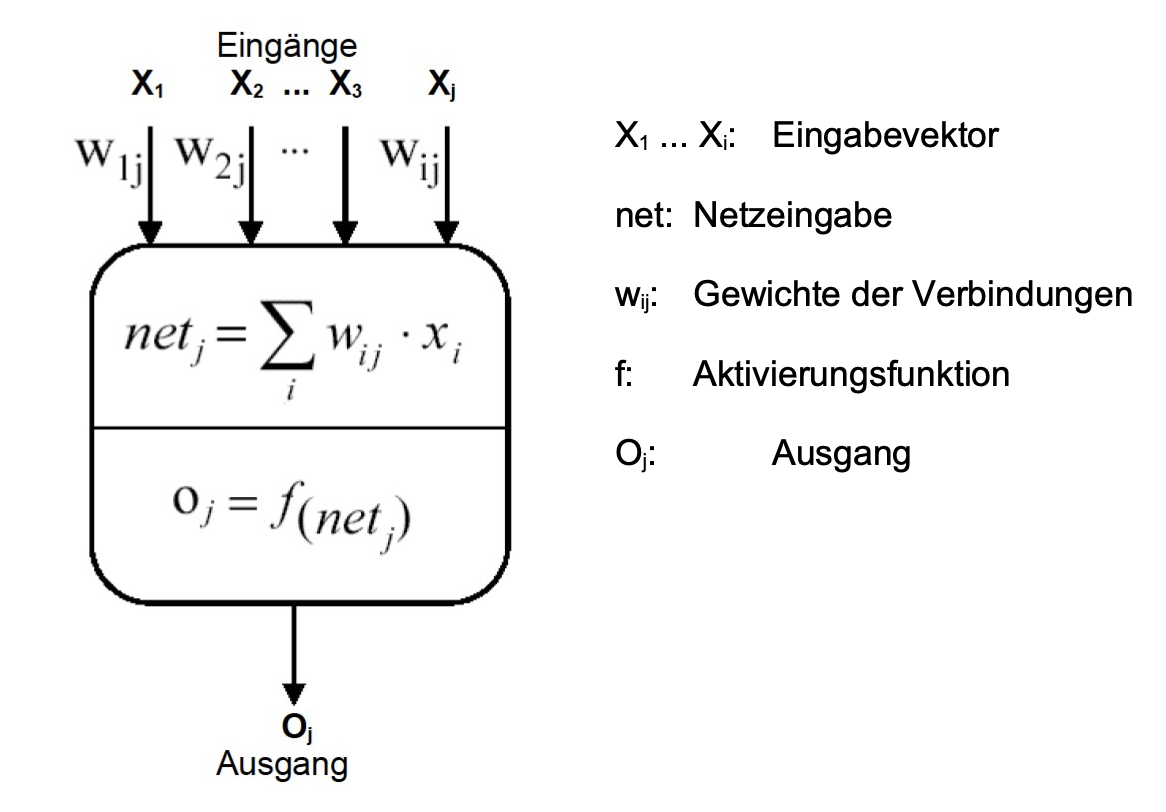
\includegraphics[width=0.4\textwidth]{images/08_durchfuehrung/nn/neuron-aufbau.png}
    \caption{Aufbau des künstlichen Neurons. Quelle: Thieling, Lothar: “Neuronale Netze (Vorlesungsskript ML)”, Kapitel F, Seite 6.}
    \label{fig:img-aufbau-neuron}
\end{wrapfigure}

Die Umwandlung in C-Code ist mögich, da ein künstliches Neuron, wie in \textbf{\autoref{fig:img-aufbau-neuron}} dargestellt, aus aus mehreren Gewichten (\textit{W\textsubscript{x}}) in Form eines Vektors besteht, der mit dem Eingabevektor (\textit{X\textsubscript{n}}) des Neurons multipliziert wird. Beide Vektoren sind Fließkommazahlen. Anschließend werden diese Produkte aufaddiert und als Eingabewert einer mathematischen Funktion, der sog. ``Aktivierungsfunktion`` (\textit{f}) verwendet. Der Ausgabewert dieser Funktion ist die Ausgabe des Neurons. \cite{neural-network-basics}

Bei einem neuronalen Netz werden die Neuronen in Schichten hinterheinander angeordnet, die Neuronen der benachbarten Schichten werden vereinfacht gesagt miteinander verbunden, also die Eingabe des einen Neurons bildet eine der Eingaben des nachfolgenden Neurons. \cite{neural-network-basics}

Sowohl die Multiplikation von Vektoren, als auch die Berechnung von Funktionswerten ist in der Programmiersprache C problemlos möglich.

Der ressourcenintensive Teil des Umgangs mit neuronalen Netzen ist das Training, also der Anpassung der Gewichtswerte bis das Neuronale Netz akzeptable Ausgabewerte liefert \cite{neural-network-basics}. Bei diesem Prozess müssen vergleichsweise sehr viele Berechnungen durchgeführt werden. Aus diesem Grund wird das Neuronale Netz zuerst trainiert und erst dann als fertiges Modell in C-Code ungewandelt und auf dem STM32 Microcontroller betrieben. 
Dass das Neuronale Netz fortlaufend durch Benutzerinteraktion weiter trainiert wird, ist nicht vorgesehen.


\subsubsection{Ansatz für die Klassizierung von Audiodaten}
\label{sec:approach-audio-classification}
Die Audiosamples liegen als WAVE-Dateien (Dateiendung .wav) vor. Diese enthalten in der Regel pulsweitenmodulierte (PCM) Audiodaten \cite{wav-contains-pcm-data}. Da die Daten nicht komprimiert sind, gehören sie in der Audio- und Musikindustrie zu den gängigsten Dateiformaten \cite{wav-popular-file-format-music-industry}. Eine typische Samplerate für WAVE-Dateien beträgt 44,1 kHz, also 44.100 Samples pro Sekunde, wobei ein Sample in der WAVE-Datei ein quantisierter Amplitudenwert zu einem bestimmten Zeitpunkt ist \cite{wav-pcm-data}. Plottet man dies als Graph, könnte ein Audiosignal wie in \textbf{\autoref{fig:img-pcm-graph}} aussehen.


\begin{figure}[h!]
\centering
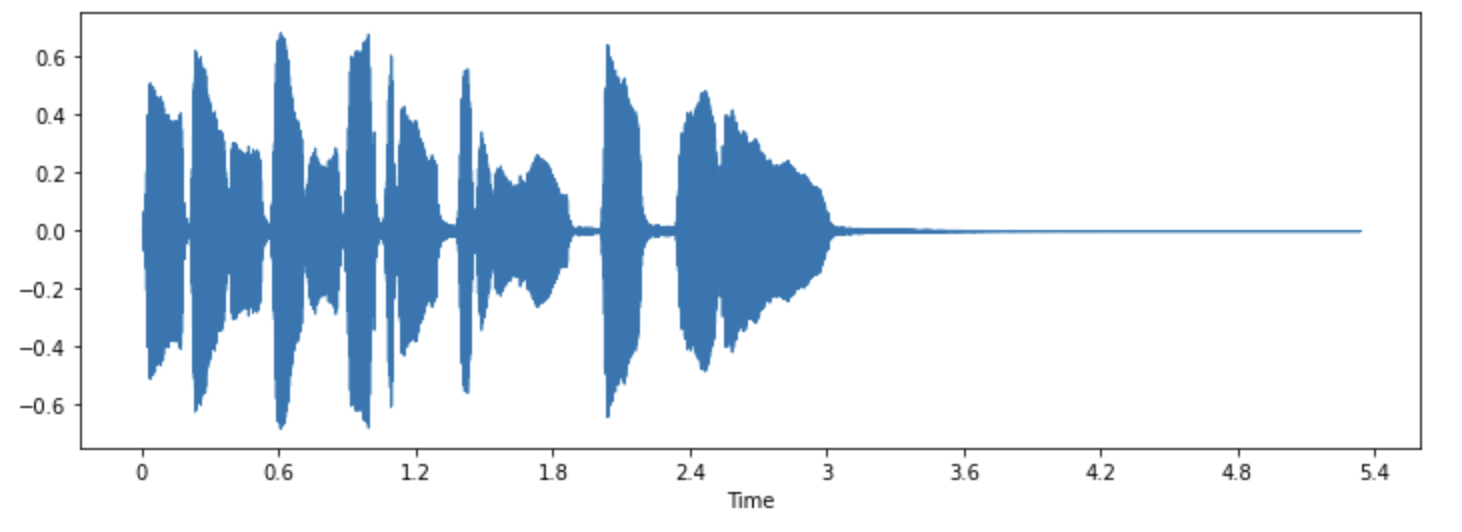
\includegraphics[width=0.6\textwidth]{images/08_durchfuehrung/nn/waveform_plot.png}
\caption{Darstellung eines PCM Audiosignals \cite{cite-img-spectrogram}}
\label{fig:img-pcm-graph}
\end{figure}

Diese Daten direkt durch ein neuronales Netz klassifizieren zu lassen, ist aus verschiedenen Gründen wenig praktikabel. Die zwei Hauptgründe sind die Merkmalsextraktion und die Größe des Eingabevektors. Letzterer Punkt würde dazu führen, dass selbst bei einer geringeren Samplerate von 16 kHz der Eingabevektor 16.000 Werte umfasst. Ein Downsampling auf eine deutlich geringere Zahl, z.B. 1000, ist aufgrund des Shannon-Nyquist-Theorems nicht praktikabel, da dieses besagt, dass die Samplerate mindestens doppelt so hoch sein muss wie die höchste Frequenz \cite{nyquist}. Damit läge der klassifizierbare Frequenzbereich nur im Bereich von \textit{0 Hz} bis maximal \textit{1000 / 2 = 500 Hz}.

Deutlich geeigneter ist es, die Daten als Spektrogramm (Amplitude der verschiedenen Frequenzen eines Signals über die Zeit) wie in \textbf{\autoref{fig:img-spectrogram}} darzustellen und mit einem Convolutional Neural Network (CNN) zu klassifizieren. CNNs werden in erster Linie zur Klassifizierung von Bildern eingesetzt. Die wesentliche Idee ist, dass das neuronale Netz dann nicht nur klassifiziert, sondern auch die Bildvorverarbeitung und die Merkmalsextraktion übernimmt \cite{how-cnn-work}. Da die Audiodateien für das menschliche Gehör klassifiziert werden, sind Mel-Spektrogramme besonders geeignet. Sie basieren auf der Mel-Skala, die das menschliche Gehör nachahmt. Die Mel-Skala ist eine nichtlineare Skala der Frequenzen, die mehr Gewicht auf tiefere Frequenzen legt \cite{mel-spectrogram}.

\begin{figure}[h!]
\centering
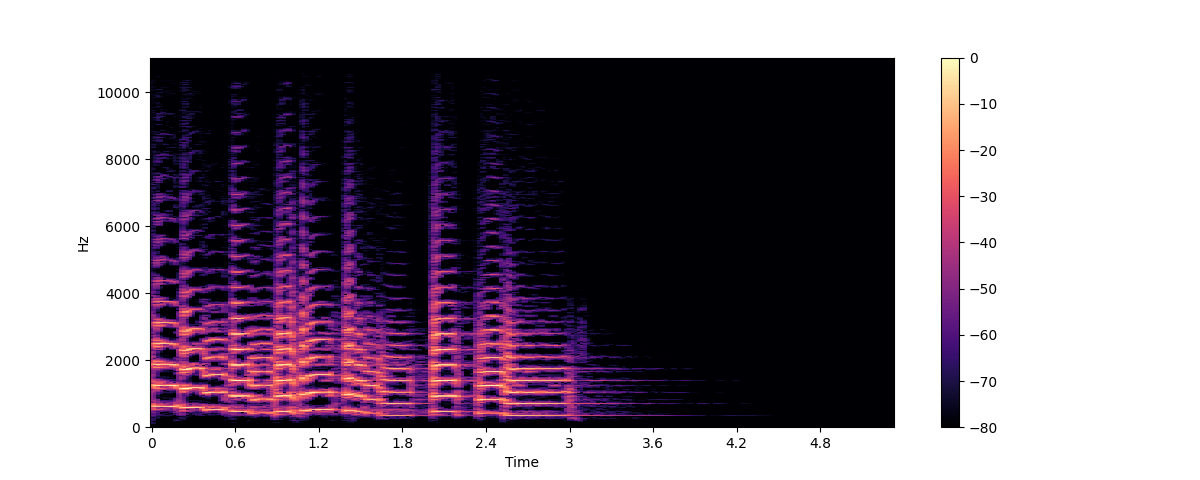
\includegraphics[width=0.75\textwidth]{images/08_durchfuehrung/nn/spectrogram_plot.png}
\caption{Darstellung eines Audiosignals als Spektrogramm \cite{cite-img-spectrogram}}
\label{fig:img-spectrogram}
\end{figure}

Der limitierende Faktor beim Einsatz eines CNN auf einem Microcontroller sind die Hardwareressourcen, also in erster Linie Flash-Speicher und RAM.

Aufgrund der fehlenden Erfahrungswerte der Teammitglieder mit der möglichen Komplexität von neuronalen Netzen, die mit den Hardwareressourcen eines Microcontrollers betrieben werden können, wird sich auf ein Beispielprojekt von STMicroelectornics gestützt. Dieses heißt ``Acoustic Scene Classification`` \cite{stm-asc}\cite{stm-asc-2}. Kern ist die Klassifizierung von 30x32 px großen Mel-Spektrogrammen mit einem zwei Schichten CNN, die einen Eingabevektor von \textit{32 x 30 = 960} Werten ergeben. 

Sowohl die Dimensionierung der Spektrogramme, als auch die Topologie des Neuronalen Netzes, die Anzahl der Neuronen je Schicht und Elemente der Datenvorverarbeitung wurden aus diesem Projekt übernommen. Damit ist sicher gestellt, dass das Neuronale Netz am Ende nicht die Ressourcen des Microcontrollers übersteigt.

Um die in \textbf{Abschnitt \ref{sec:classification-intro}} beschriebenen Merkmalsklassen zu definieren, wurden zunächst Kategorien überlegt, die für die Musikproduktion relevant sind. Anschließend wurden Spektrogramme dieser Klassen in der vorgesehenen Auflösung erstellt und analysiert. Ziel war es zu prüfen, ob das menschliche Auge bzw. Gehirn in der Lage ist, die Merkmalsklassen anhand der Spektrogramme zu differenzieren. Diese Überprüfung diente dazu, die grundsätzliche Machbarkeit der Klassifikation in die Merkmalsklassen durch das neuronale Netz zu bestätigen.


\subsubsection{Generieren der Eingabedaten}
\label{sec:input-data-generation}
Für das Training des neuronalen Netzes sind Trainingsdaten erforderlich. Diese bestehen aus Eingabedaten, die bereits mit den korrekten Klassifikationsergebnissen, also Labels, versehen sind. Um das Training des neuronalen Netzes während des Trainings einschätzen und nach Abschluss des Trainings validieren zu können, werden die Eingabedaten in drei Segmente aufgeteilt.

Da online keine kostenlosen und bereits mit den passenden Labels versehene Datensätze gefunden werden konnten, wurden eigene Daten generiert. Grundlage hierfür bildet eine private Audiosample-Bibliothek. Ein eigens entwickeltes Python-Skript ermöglicht es, Audiosamples auszuwählen, abzuspielen und zeiteffizient zu labeln.

\begin{figure}[h!]
	\centering
	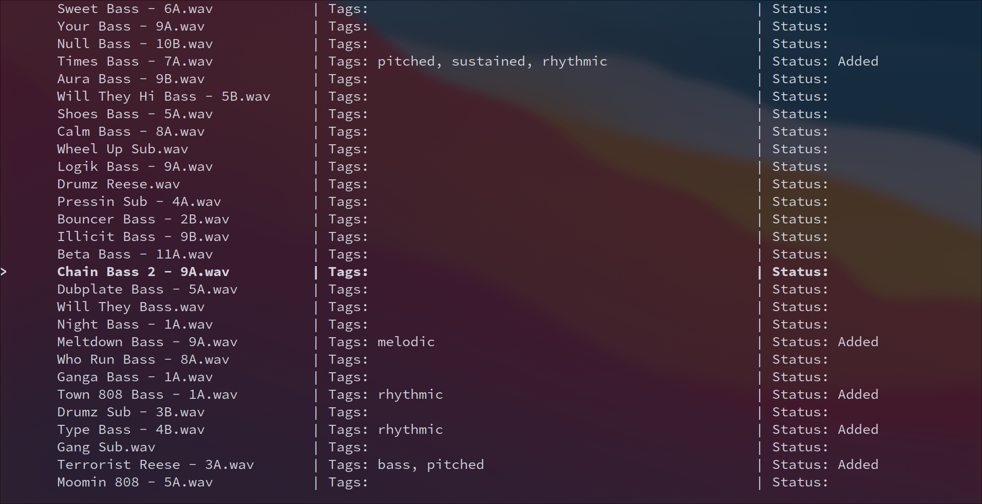
\includegraphics[width=0.75\textwidth]{images/08_durchfuehrung/nn/training_script_screenshot.png}
	\caption{Python Script zum manuellen Tagging der Trainingsdaten}
	\label{fig:training_script_screenshot}
\end{figure}

Für jedes manuell gelabelte Audiosample wird eine eindeutige Identifikationsnummer (UID) generiert. Die zugehörigen Labels werden in einer CSV-Datei gespeichert. Ein Beispiel für einen solchen Datensatz zeigt \textbf{\autoref{tab:audiodaten}}. Außerdem wird eine Kopie des Audiosamples unter dem Namen der UID im Ausgabeordner des Skripts abgelegt. Diese Dateien werden später vom Jupyter-Notebook für das Training verwendet.

\begin{table}[h!]
\centering
\begin{tabular}{|m{2.8cm}|m{4.5cm}|m{0.8cm}|m{1.2cm}|m{1.5cm}|m{1.5cm}|m{1.3cm}|}
\hline
\textbf{UID} & \textbf{File} & \textbf{bass} & \textbf{pitched} & \textbf{sustained} & \textbf{rhythmic} & \textbf{melodic} \\ \hline
ecfad96b740844c3
9c96127279f22cf6 &  BD 606 Long MPC60 01.wav & 1 & 0 & 0 & 1 & 0 \\ \hline
\end{tabular}
\caption{Beispielhafter Datensatz eines Audiosamples}
\label{tab:audiodaten}
\end{table}

Bei der Auswahl der Audiosamples wurde darauf geachtet, dass die Daten annähernd gleich verteilt sind, um eine ausgewogene Trainingsbasis zu schaffen. Ein Ungleichgewicht in den Daten kann sich negativ auf das Training und die Klassifikationsergebnisse auswirken. Überrepräsentierte Merkmale könnten die Klassifikationsschwellenwerte beeinflussen, sodass die häufiger vorkommenden Klassen später bevorzugt erkannt werden \cite{nn-imbalance-input-data}. Wie in \textbf{\autoref{fig:img-class-spread-graph}} zu sehen, ist die Gleichverteilung jedoch zugegebenermaßen nur begrenzt gelungen, mit deutlich überrepräsentierten Eingabedaten mit dem Merkmal "melodic".

\begin{figure}[h!]
\centering
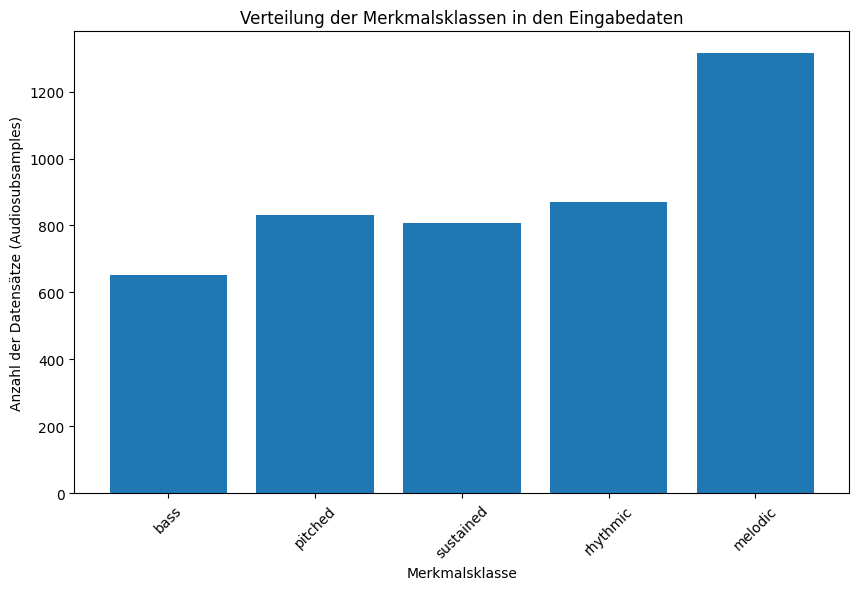
\includegraphics[width=0.75\textwidth]{images/08_durchfuehrung/nn/class_spread_plot.png}
\caption{Repräsentation der verschiedenen Merkmalsklassen in den Entwicklungsdaten}
\label{fig:img-class-spread-graph}
\end{figure}

Zudem wurde versucht sicherzustellen, dass der Variationsbereich jeder Klasse möglichst umfassend abgedeckt ist. Dies umfasst sowohl reine Formen jeder Klasse – beispielsweise bei „pitched“ Audiosamples ausschließlich mit Tönen aus dem hohen Frequenzbereich – als auch Mischformen, die Merkmale mehrerer Klassen kombinieren.

Insgesamt wurden 209 Audiosamples unterschiedlicher Länge mit Labels versehen.

\subsubsection{Datenvorverarbeitung}
\label{sec:data-preprocessing}

Für die Datenvorverarbeitung und das Training des neuronalen Netzes wird ein Jupyter-Notebook verwendet. Dieses ermöglicht eine Kombination aus formatiertem Text und Code, in diesem Fall Python, was die Lesbarkeit und Nachvollziehbarkeit des Codes erleichtert.

Damit die gelabelten Daten für das Training des neuronalen Netzes verwendet werden können, müssen sie zunächst aufbereitet bzw. vorverarbeitet werden. Um die zu verarbeitenden Datenmengen sinnvoll zu verringern, wird zunächst die Samplerate aller Audiosamples auf 16 kHz reduziert.

Wie im \textbf{Abschnitt \ref{sec:input-data-generation}} erwähnt, liegen die Audiosamples als WAVE-Dateien unterschiedlicher Längen vor. Die in \textbf{Abschnitt \ref{sec:approach-audio-classification}} beschriebenen Dimensionen der durch das neuronale Netz klassifizierbaren Mel-Spektrogramme betragen 32x30 Pixel. Um bei unterschiedlich langen Audiosamples die zeitliche Abhängigkeit zu bewahren und auch bei längeren Audiosamples wichtige Informationen im Spektrogramm abzubilden, müssen die Audiosamples in Sektionen gleicher Länge unterteilt werden, wobei später aus jeder Sektion ein Spektrogramm erstellt wird. Diese Sektionen werden im Folgenden als „Audiosubsamples“ bezeichnet.

Aus den in \textbf{Abschnitt \ref{sec:input-data-generation} }erwähnten 209 gelabelten Audiosamples wurden durch deren Aufteilung insgesamt 2.837 Audiosubsamples gewonnen.

Ein Audiosubsample, also ein Mel-Spektrogramm, entspricht dabei 16.896 Samples, was bei einer Samplerate von 16 kHz etwas mehr als einer Sekunde entspricht. Analog zum Beispielprojekt „Acoustic Scene Classification“ \cite{stm-asc}\cite{stm-asc-2} werden die Audiosubsamples anschließend mittels eines „Sliding Window“ in 1024 Samples lange, um 512 Samples überlappende, Frames unterteilt.  Diese Überlappung stellt sicher, dass Informationen zu den Anfangs- und Endzeitpunkten der Frames nicht durch das „Abschneiden“ verloren gehen. Aus den 16.896 Samples eines Audiosubsamples lassen sich dadurch 32 Frames gewinnen. Die Aufteilung der Audiosamples in Audiosubsamples und Frames wird in \textbf{\autoref{fig:img-audiosubsamples-frames-overview}} visualisiert.

\begin{figure}[h!]
\centering
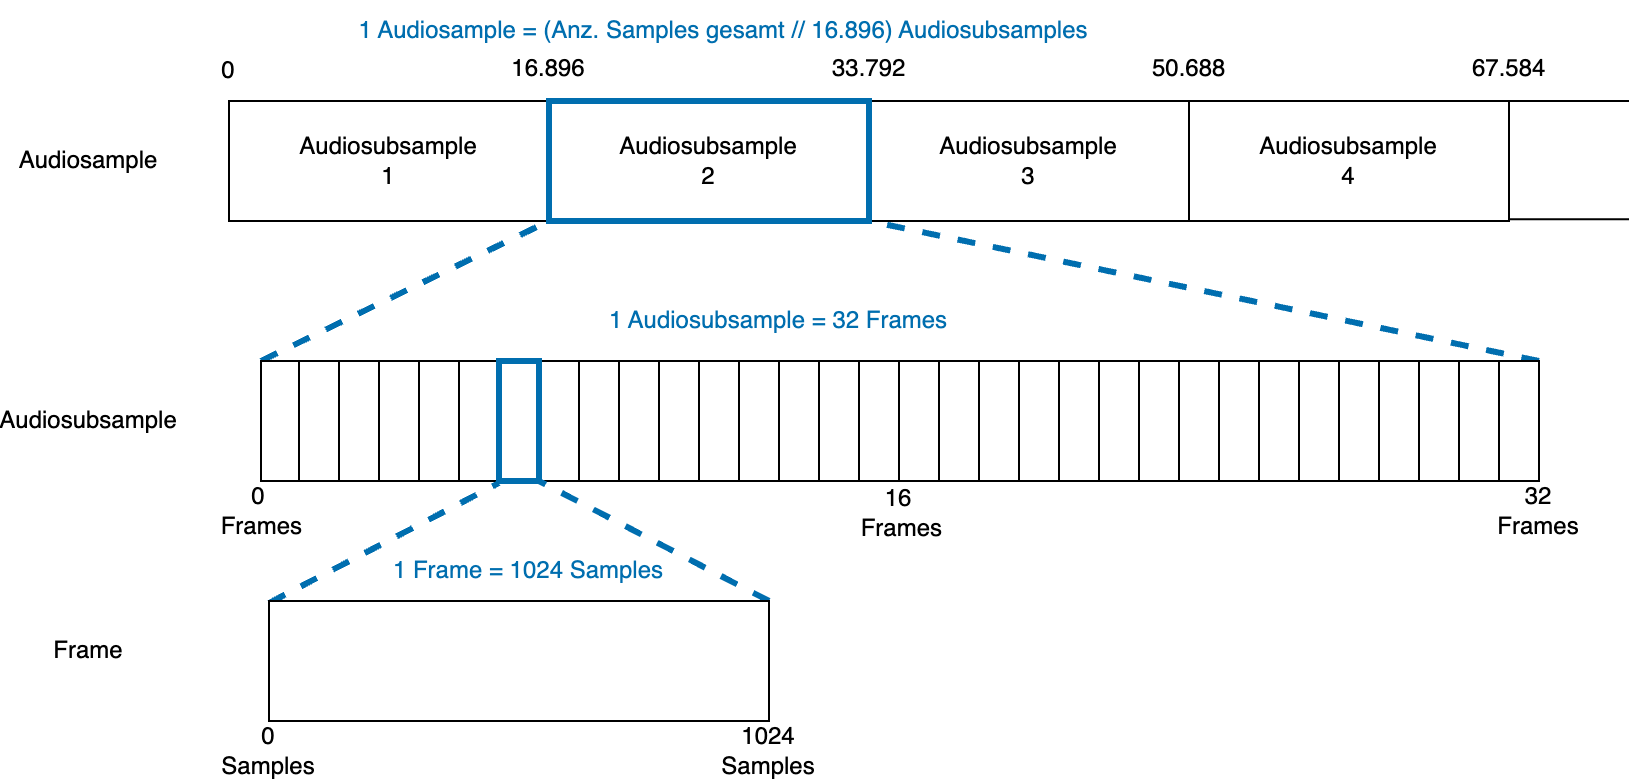
\includegraphics[width=0.8\textwidth]{images/08_durchfuehrung/nn/audiosubsamples_frames_overview.png}
\caption{Darstellung der Unterteilung der Audiosamples in Audiosubsamples und Frames}
\label{fig:img-audiosubsamples-frames-overview}
\end{figure}

Das Sliding Window Prinzip, mit dem Audiosubsamples in überlappende Frames unterteilt werden, ist in \textbf{\autoref{fig:img-sliding-window}} dargestellt.

\begin{figure}[h!]
\centering
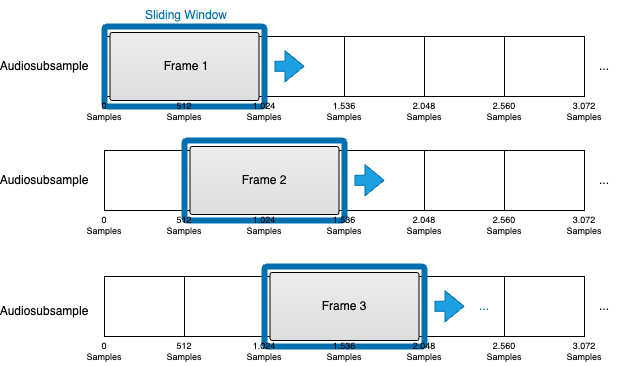
\includegraphics[width=0.7\textwidth]{images/08_durchfuehrung/nn/sliding_window.png}
\caption{Darstellung des Sliding Window Prinzips}
\label{fig:img-sliding-window}
\end{figure}

Nun können die Mel-Spektrogramme erstellt werden. Eine Spalte des Spektrogramms wird dabei aus einem Frame berechnet. Setzt man die 32 in einem Audiosubsample enthaltenen Frames, also Spektrogramm-Spalten, zusammen, erhält man das 32x30 Pixel große Spektrogramm für ein Subsample.

Abschließend müssen die erhaltenen Daten standardisiert, also mittelwertfrei gemacht werden. Dies ist bei maschinellen Lernen üblich und trägt dazu bei, dass das Modell schneller und effizienter konvergiert. Durch die Reduzierung der Varianz in den Eingabedaten und die Sicherstellung einer gleichmäßigen Verteilung der Werte verbessert sich die Modellleistung \cite{ml-standardization-reason}. Um diese Standardisierung auch später beim Einsatz des neuronalen Netzes auf dem Mikrocontroller nachzuahmen, werden die Werte des Scalers, der zur Berechnung der standardisierten Werte verwendet wird, exportiert. Bei den Werten des Scalers handelt es sich um Fließkommazahlen, jeweils eine für jeden Eingabevektorwert. Diese Werte werden dann später mit den Eingabevektorwerten multipliziert, um den standardisierten Wert zu simulieren.


\subsubsection{Aufteilen der Eingabedaten in Trainings- Test und Validierungsdaten}
Wie in \textbf{Abschnitt \ref{sec:input-data-generation} }beschrieben, wurden 209 Audiosamples mit Labeln versehen. Diese  in 2.837 Audiosubsamples aufgeteilt. Für das Training des neuronalen Netzes werden die Daten wie üblich in Trainingsdaten, Validierungsdaten und Testdaten aufgeteilt \cite{ml-data-splitting-reason}.

\textbf{Trainingsdaten} (1.701 Datensätze) werden direkt für das Training des neuronalen Netzes genutzt.

\textbf{Validierungsdaten} (568 Datensätze) dienen dazu, den Fortschritt und Erfolg des Trainings über die verschiedenen Durchläufe (Epochen) hinweg zu überwachen.

\textbf{Testdaten} (568 Datensätze) werden nach dem Abschluss des Trainingsvorgangs eingesetzt, um die Genauigkeit und Zuverlässigkeit der Klassifikation zu bewerten.

Eine Visualisierung der Datenaufteilung ist in \textbf{\autoref{fig:img-input-data-graph}} dargestellt.

\begin{figure}[h!]
\centering
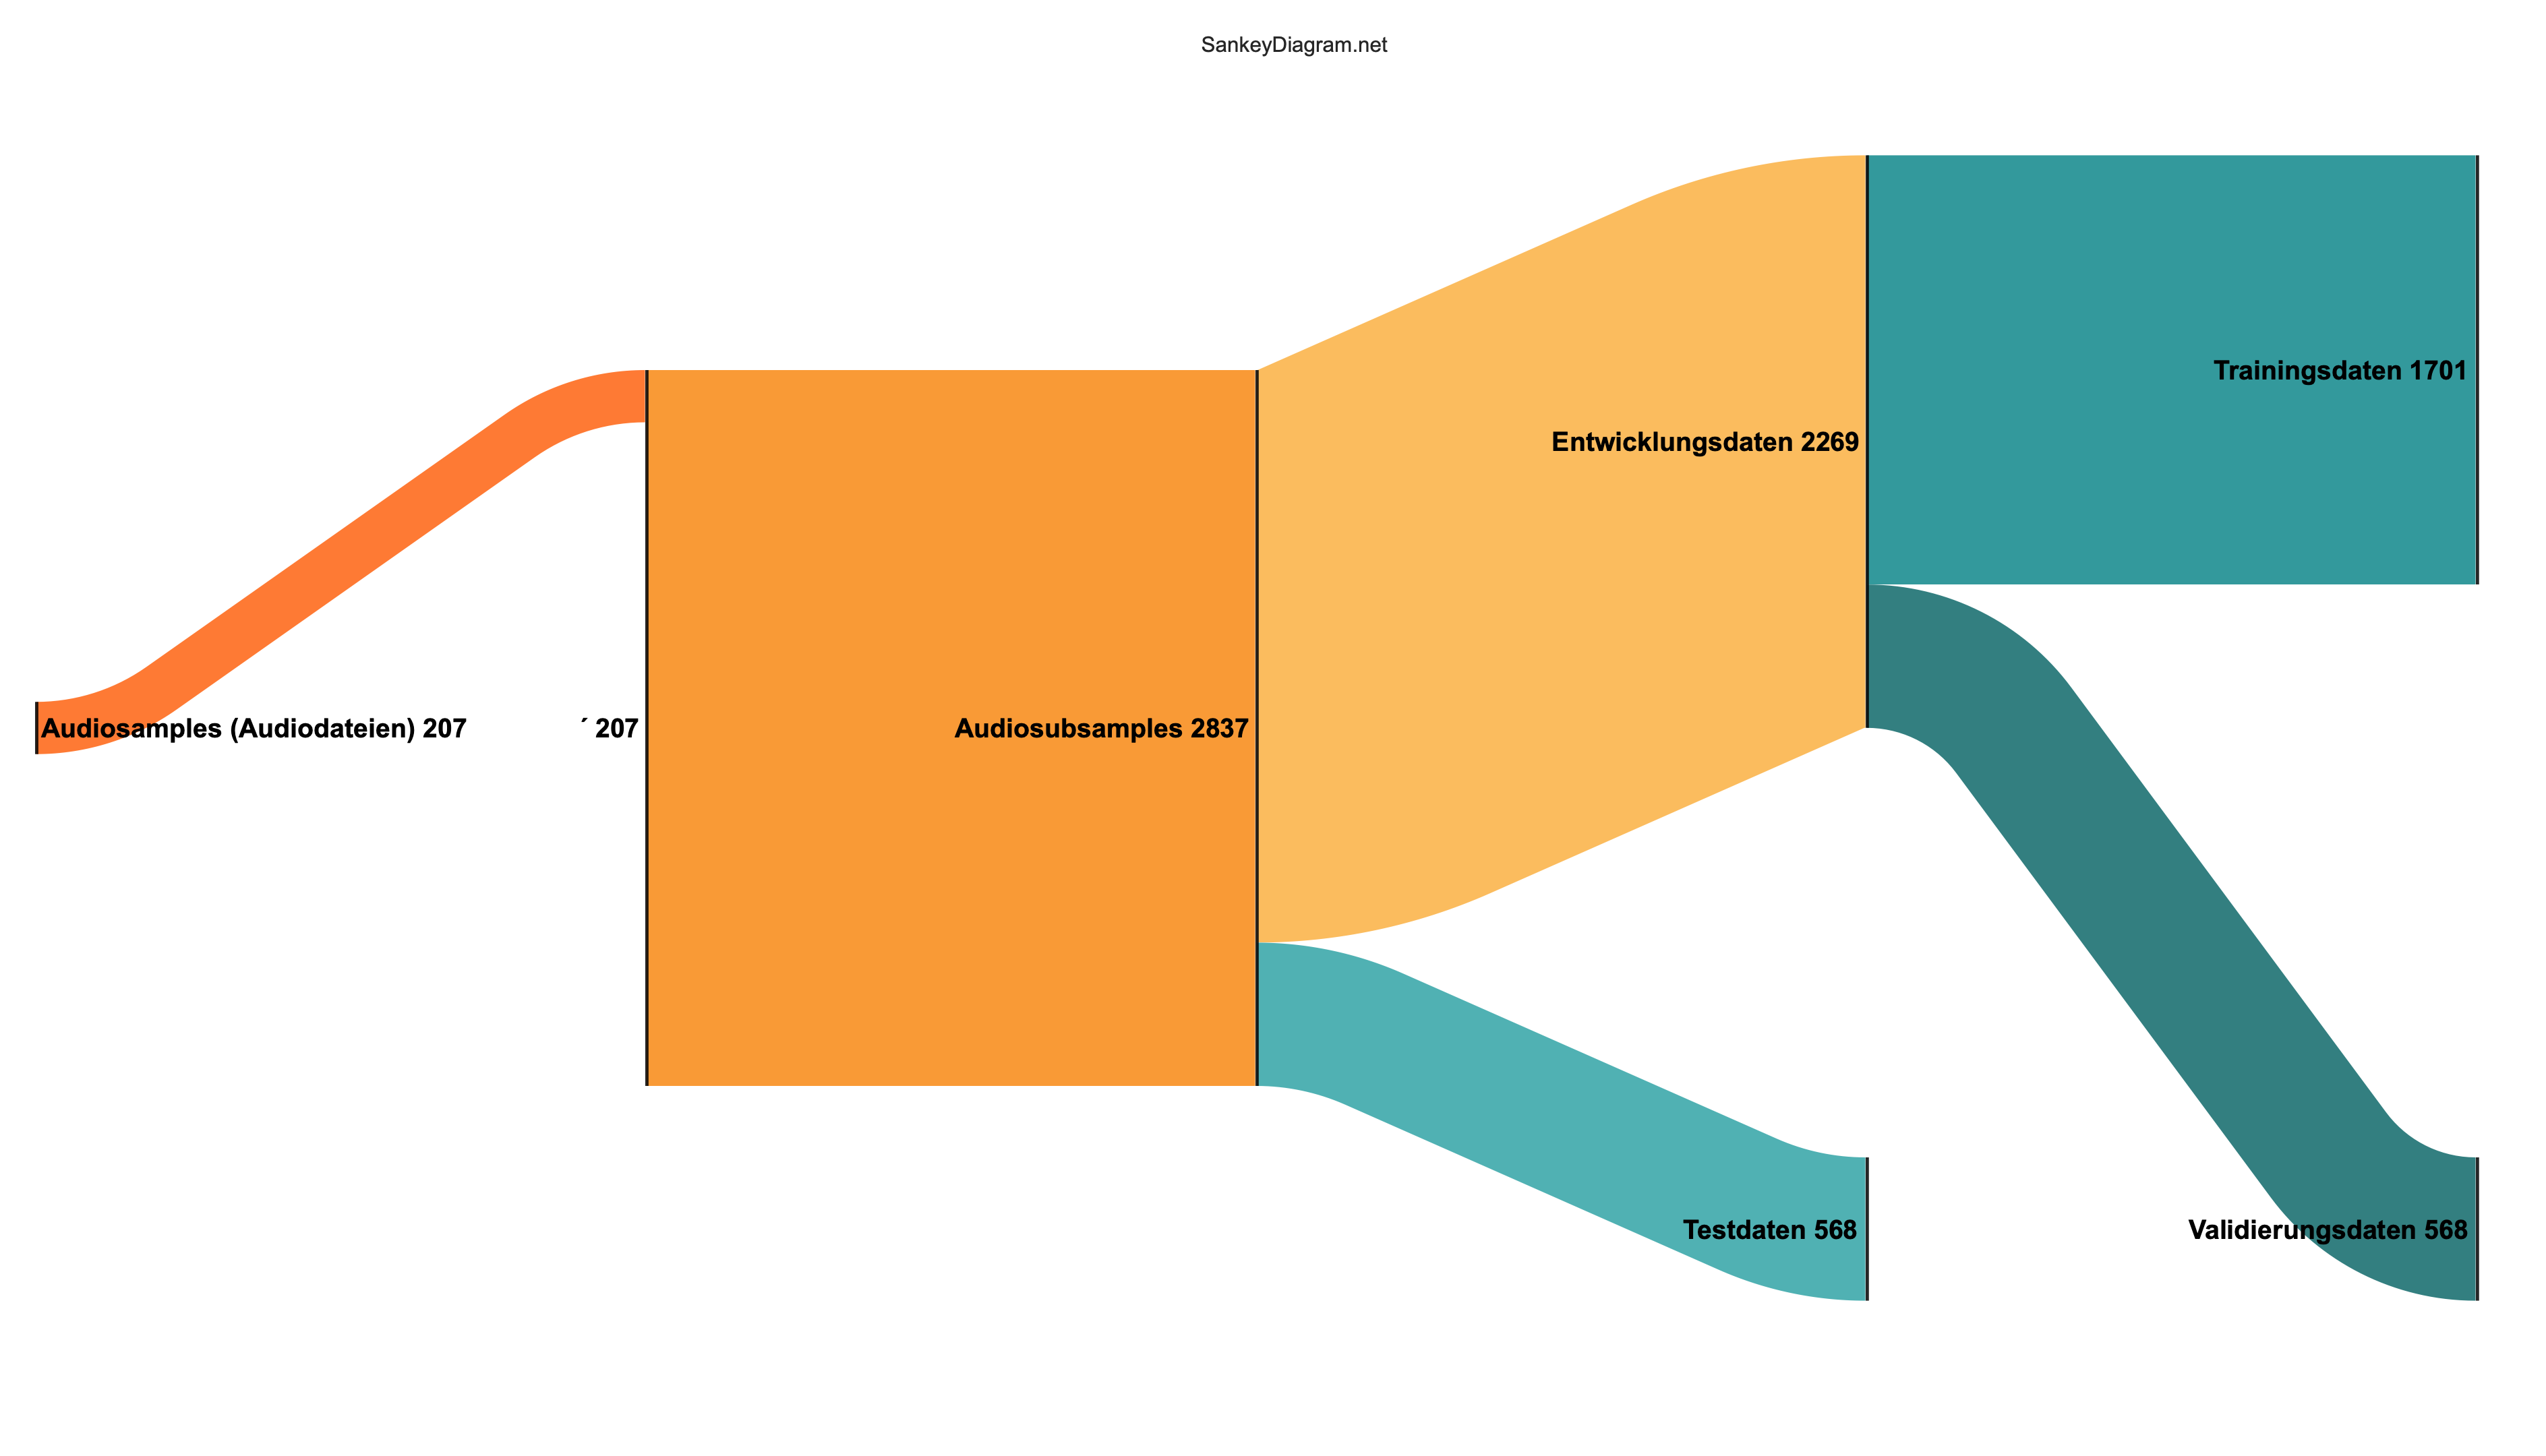
\includegraphics[width=0.95\textwidth]{images/08_durchfuehrung/nn/input-data-graph.png}
\caption{Aufteilung der Eingabedaten in Trainings- Validierungs- und Testdaten (erstellt mit sankeydiagram.net)}
\label{fig:img-input-data-graph}
\end{figure}

\subsubsection{Training des neuronalen Netzes}

Nach der Datenvorverarbeitung beginnt das eigentliche Training des neuronalen Netzes. Typischerweise bestehen Convolutional Neural Networks (CNNs) aus mehreren Faltungsschichten (Convolutional Layers), die der Vorverarbeitung der Eingabedaten und der Merkmalsextraktion dienen. Die Faltungsmasken, die über das Eingabebild gefaltet werden, stellen die Neuronen dar, die trainiert werden. Jede Faltungsschicht wird in der Regel von einer Pooling-Schicht (Pooling Layer) gefolgt, welche die Datenmenge reduziert und die Dimensionalität des Ausgabebildes sinnvoll verkleinert. \cite{how-cnn-work}

``Normale`` neuronale Netze, oft als ``Dense`` oder ``Fully Connected Networks`` bezeichnet, können nur Vektoren verarbeiten. Eine sogenannte ``Flattening``-Schicht wandelt die zweidimensionale Ausgabematrix des CNNs in einen eindimensionalen Vektor um. Nach dieser Transformation übernehmen zwei ``Dense-Layers`` die eigentliche Klassifikation. An der Ausgabe des zweiten Dense-Layers, die einen Vektor mit fünf Werten zurückgibt, kann das Klassifikationsergebnis abgelesen werden. \cite{how-cnn-work}

Im folgenden Codeausschnitt des Jupyter-Notebooks wird die Struktur des neuronale Netzes definiert. Die Parameter der \mintinline{python}|add|-Funktion beziehen sich auf die Art der Schicht, der Anzahl bzw. Dimensionierung der Ausgabematrix und die Aktivierungsfunktion.

\begin{minted}{python}
model = models.Sequential()
model.add(layers.Conv2D(16, (3, 3), activation='relu', 
		input_shape=(30, 32, 1), data_format='channels_last'))
model.add(layers.MaxPooling2D((2, 2)))
model.add(layers.Conv2D(16, (3, 3), activation='relu'))
model.add(layers.MaxPooling2D((2, 2)))
model.add(layers.Flatten())
model.add(layers.Dense(25, activation='relu'))
model.add(layers.Dense(5, activation='sigmoid'))	
\end{minted}

Bei der Aktivierungsfunktion ist zu beachten, dass bei allen Schichten des CNNs sich die ReLu Funktion und deren Abwandlungen (z.B. Leaky-ReLu) bewährt haben, da sie die Performance des Modells aus unterschiedlichen Gründen verbessern. In den Dense-Layern, insbesondere in der Ausgabeschicht, ist die sigmoidale Aktivierungsfunktion besonders geeignet, da sie die Ergebnisse der einzelnen Ausgabeneuronen als Ähnlichkeiten interpretiert. Diese Ähnlichkeiten liegen im Bereich zwischen 0 und 1 und sind ideal für mehrklassige Klassifikationsaufgaben, bei denen jedes Ausgabeneuron eine Merkmalsklasse repräsentiert. \cite{cnn-relu-sigmoid}

In der folgenden Zeile Code geschieht das Training des zuvor definierten neuronalen Netzes durch.

\begin{minted}{python}
history = model.fit(x_train_r, y_train, validation_data=(x_val_r, y_val),
                    batch_size=1, epochs=100, verbose=2)
\end{minted}

\begin{mdframed}

\textbf{x\_train\_r}: Eingabedaten, die für das Training des Modells verwendet werden.

\textbf{y\_train}: Soll-Ausgabedaten (Labels), die die tatsächlichen Klassen der Trainingsdaten repräsentieren.

\textbf{validation\_data}: Validierungsdaten (x\_val\_r) und zugehörige Labels (y\_val). Sie dienen dazu, die Klassifierung des Modells zu überprüfen und zu verhindern, dass das Modell einfach nur die Trainingsdaten ``auswendig lernt`` (Overfitting).

\textbf{batch\_size}: Anzahl der Datensätze, die durch das neuronale Netz verarbeitet werden, bevor eine Gewichtsanpassung der Neuronen erfolgt. Eine Batch-Size von 1 bedeutet, dass nach jedem Datensatz die Gewichte aktualisiert werden, was dem sogenannten Stochastic Gradient Descent entspricht.

\textbf{epochs}: Gibt an, wie oft der gesamte Satz der Trainingsdaten durch das Modell verarbeitet wird. Hier werden die Trainingsdaten insgesamt 100 Mal durchlaufen.

\end{mdframed}

\begin{wrapfigure}{r}{0.4\textwidth} % Increase the width of the figure environment
	\vspace{-20pt + 0.02\textwidth}
	\fbox{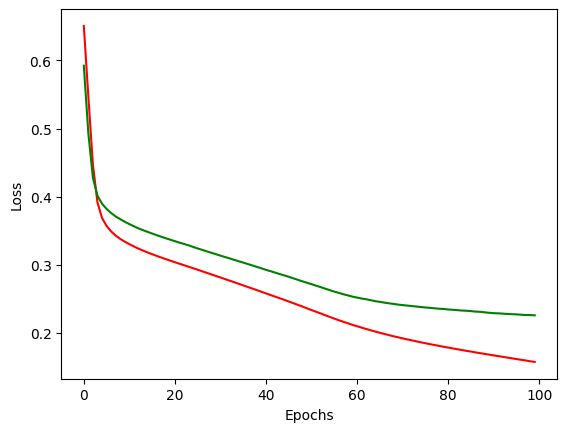
\includegraphics[width=0.4\textwidth]{images/08_durchfuehrung/nn/nn_learning_curve.png}}
	\caption{Darstellung des Loss-Werts über den Verlauf der Epochen}
	\label{fig:img-training-graph}
\end{wrapfigure}

\textbf{\autoref{fig:img-training-graph}} veranschaulicht, wie sich der ``Verlust-Wert`` (Loss) während des Trainingsprozesses des neuronalen Netzes über die Epochen hinweg verändert. Der rote Graph repräsentiert die Trainingsdaten und der grüne Graph die Validierungsdaten. Der Loss-Wert gibt an, wie stark die Vorhersagen des Netzwerks von den tatsächlichen Daten abweichen. Eine hohe Abweichung bedeutet, dass das Netzwerk nicht gut vorhersagt, während eine niedrige Abweichung auf bessere Vorhersagen hinweist.

Wie sich erkennen lässt, ``lernt`` das neuronale Netz im Laufe der Epochen, die Eingabedaten besser zu klassifizieren, was sich in einem sinkenden Loss-Wert niederschlägt. Da der Loss-Wert der Validierungsdaten ebenfalls sinkt, ist gewährleistet, dass das neuronale Netz nicht einfach nur die Trainingsdaten auswendig lernt, sondern tatsächlich generalisiert.

Abschließend kann das trainierte Modell als ``Tensorflow-Lite``-Dateiformat (Dateiendung ``.tflite``) exportiert werden. Die ``model.tflite``-Datei enthält sowohl die Architektur, als auch die Gewichte der einzelnen Neuronen \cite{tflite-file}.

\subsubsection{Betrieb des neuronalen Netzes auf dem STM32 Microcontroller}

Für den Betrieb des Neuronalen Netzes wird ``STM32Cube.AI`` verwendet, um das in der ``model.tflite`` Datei definierte Neuronale Netz in C-Code nachzubilden. Um jedoch Audiodateien klassifizieren zu können, müssen zunächst sämtliche Schritte der Datenvorverarbeitung, die im Jupyter-Notebook gemacht wurden, wiederholt werden.

\textbf{Einlesen der Datei und Datenvorverarbeitung}


Zum Einlesen der Datei wird die in \textbf{Abschnitt \ref{sec:audio-downsampling}} beschriebene Funktion \mintinline{c}|downsample_1024_samples()| verwendet. Diese reduziert die Datenmenge um den Faktor 3, was bei einer Eingabe-Samplerate von 44.1 kHz zu einer Ausgabe-Samplerate von 14.700 kHz (statt 16.000 kHz) führt. Die resultierende Abweichung von $\approx$ 8.8\% wird jedoch als vernachlässigbar für das Klassifikationsergebnis eingeschätzt.

Für die Berechnung der Mel-Spektrogramme wird die Bibliothek ``STM32\_AI\_AudioPreprocessing\_Library`` verwendet. Diese ist Teil des ``FP-AI-SENSING1`` Function Packs \cite{fp-ai-sensing1}. Mit dieser lassen sich einzelne Spektrogrammspalten berechnen, deren Amplitudenwerte müssen jedoch im Anschluss noch in Dezibel (dB) umgerechnet werden.

\textbf{Übersetzen des neuronalen Netzes mit STM32Cube.AI}


\begin{wrapfigure}{r}{0.4\textwidth} % Increase the width of the figure environment
	\vspace{-20pt + 0.02\textwidth}
	\hspace{0.02\textwidth} % Add horizontal space
	\fbox{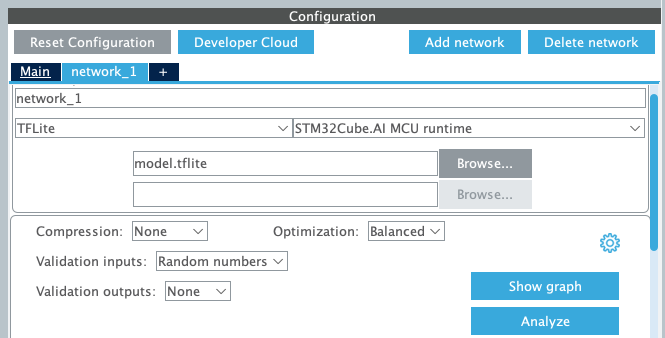
\includegraphics[width=0.4\textwidth]{images/08_durchfuehrung/nn/cube_ai_config.png}}
	\caption{Konfiguration von STM32Cube.AI in CubeMX}
	\label{fig:img-training-graph}
\end{wrapfigure}

Für die Nutzung von STM32Cube.AI muss zunächst in der CubeMX-Datei das Software Package ``X-CUBE-AI`` in Version 9.0.0 heruntergeladen werden. Im Reiter ``Configuration`` lässt sich ein Name für das Modell festlegen, welcher später im Code zur Referenzierung verwendet wird. Hier wird ebenfalls die Modell-Datei ``model.tflite`` eingebunden. Durch einen Klick auf ``Analyze`` wird das Modell in C-Code übersetzt und ein Bericht zur Ressourcennutzung erstellt. Dieser bestätigt, dass die Ressourcenlimits des verwendeten Nucleo-Boards eingehalten werden. Der folgende Auszug gibt einen Überblick über die genutzten Ressourcen:

\begin{minted}{text}
Total Flash		82.050 B (80.13 KiB)
Total Ram  		21.844 B (21.37 KiB)
\end{minted}



\textbf{Nutzung von STM32Cube.AI}

Die Nutzung von STM32Cube.AI wird anhand eines Beispiels in der Dokumentation beschrieben \cite{stm32-cube-ai-documentation}. Obwohl das Beispiel auf einer älteren Version basiert, hat sich der grundlegende Umgang mit der Software nicht verändert. Da die Nutzung der Funktionen und Zeck der einzelnen Variablen dort im Detail  beschrieben sind, wird dies im folgenden Abschnitt nur kurz zusammengefasst.

Zur Nutzung von STM32Cube.AI ist ein Handle vom Typ \mintinline{c}|ai_handle| erforderlich. Dieses erhält man durch den Aufruf der Initialisierungsfunktion \mintinline{c}|ai_network_1_create_and_init()|. Anschließend werden Input- und Outputbuffer vom Typ \mintinline{c}|ai_buffer| initialisiert, die zur Eingabe von Daten in das neuronale Netz und zur Rückgabe des Klassifikationsergebnisses verwendet werden. Diese Initialisierungsschritte werden im Code des Projekts in der Funktion \mintinline{c}|init_nn()| durchgeführt:

\begin{minted}{c}
int init_nn() {
	ai_error err;
	const ai_handle act_addr[] = { activations };

	err = ai_network_1_create_and_init(&network, act_addr, NULL);
	if (err.type != AI_ERROR_NONE) { return -1; }
	
	ai_input = ai_network_1_inputs_get(network, NULL);
	ai_output = ai_network_1_outputs_get(network, NULL);

	return 0;
}
\end{minted}

Hat man den Handle, kann man Daten durch das neuronale Netz klassifizieren lassen. Dazu müssen zunächst Pointer auf die Eingabe- bzw. Ausgabedaten in das \mintinline{c}|data| Feld der Input- und Outputbuffer gesetzt werden. Die Klassifizierung wird durch den Aufruf der Funktion \mintinline{c}|ai_network_1_run()| initiiert. Das Ergebnis der Klassifizierung wird anschließend in der Variable verfügbar, die durch den zuvor übergebenen Output-Pointer referenziert wurde. Dieser Prozess ist im Code in der Funktion \mintinline{c}|run_nn_classification| implementiert. Da vor der Klassifizierung die Standardisierung mit den exportierten Scaler-Werten erforderlich ist, wird diese in der Funktion vor dem Klassifizierungsvorgang umgesetzt.

\begin{minted}{c}
int run_nn_classification(ai_float* pSpectrogram, ai_float* classification_result) {
    ai_i32 batch;
    ai_error err;

    ai_input[0].data = AI_HANDLE_PTR(pSpectrogram);
    ai_output[0].data = AI_HANDLE_PTR(classification_result);

    if (network == AI_HANDLE_NULL) { return -1; }

    for (int i = 0; i < AI_NETWORK_1_IN_1_SIZE; i++) {
    	pSpectrogram[i] = (pSpectrogram[i] - feature_scaler_mean[i]) / feature_scaler_std[i];
    }

    batch = ai_network_1_run(network, ai_input, ai_output);
    if (batch != 1) { return -1; }

    return 0;
}
\end{minted}

\textbf{Erfahrungswerte bei der Nutzung von STM32Cube.AI}

Insgesamt konnte für die Klassifikation eines Spektrogramms, also eines Audiosubsamples, eine Inferenz von 17 ms gemessen werden. Die Inferenz gibt an, wie viel Zeit die Klassifizierung eines Datensatzes benötigt.

Während der Nutzung von STM32Cube.AI trat im Projektverlauf ein ``HardFault``-Fehler bei der Ausführung der Funktion \mintinline{c}|ai_network_1_run()| auf. Dies konnte darauf zurückgeführt werden, dass eine fehlerhafte Deklaration einer Variable im Header der aktuellen Datei vorlag. Sie war nicht als \mintinline{c}|extern| gekennzeichnet. Obwohl die aufgerufene externe STM32Cube.AI-Bibliothek nicht direkt auf diese Variable zugriff, führte das Fehlen der extern-Deklaration vermutlich zu einer inkonsistenten Referenz beim Linken der Module.

Leider konnte die Klassifizierung durch das neuronale Netz aus zeitlichen Gründen nicht in das Gesamtprojekt integriert werden. Daher sind für die Komponente ``Neuronales Netz`` im Anhang zwei CubeMX-Projekte enthalten:

\begin{itemize}
\item \textbf{esp\_cubeai\_test}: Dieses Projekt diente der Überprüfung und Validierung der Funktionen von STM32Cube.AI, der Spektrogramm-Berechnungsbibliothek sowie der selbst entwickelten Funktionen für das Aufteilen in Frames. Als Datenbasis dient ein Audiosubsample, das in einer C-Datei als 16.896 \mintinline{c}|short|-Werte gespeichert ist. Dadurch konnte der Ablauf der Klassifikation unabhängig von anderen Komponenten getestet werden. Weitere Details zur Validierung und zu den Tests sind im \textbf{Abschnitt \ref{sec:test-validation}} zu finden.
\item \textbf{esp\_cubeai\_for\_integration}: Dieses Projekt enthält Code, der für die Integration in das Gesamtprojekt vorbereitet und strukturiert wurde. Der Code wurde jedoch noch nicht getestet und könnte Fehler enthalten. Zusätzlich wurde das Auffüllen von Audiosamples (``zero-padding``), die weniger als 16.896 Samples enthalten, noch nicht implementiert.
\end{itemize}
